\chapter{CNN Architectures}%
\label{chap:04}

\paragraph{Summary} This week, we discuss two particular variants of
convolutional neural networks. The first is AlexNet, one of the most influential
networks that was one of the first CNNs to outperform traditional methods in an
image classification challenge. The second is a network for semantic
segmentation, called the UNet. As part of improving UNet's performance, we also
discuss two normalisation techniques.

\section{Convolutional Neural Networks (CNNs) for Image Classification}
In 2012, the convolutional neural network AlexNet achieved an outstanding
performance on the ImageNet Visual Recognition Challenge, scoring more than 10
percentage points lower in the top-5 error than the runner up. The associated
research paper has been cited more than 60,000 times and is considered one of
the most influential papers in computer vision. In the same year of the AlexNet
publication, deep neural networks started to supersede and replace traditional
methods.

The following image shows the structure of the VGG16 network. It can be seen as
an improvement of AlexNet but the overall structure is very similar.
\begin{figure}[H]
  \centering 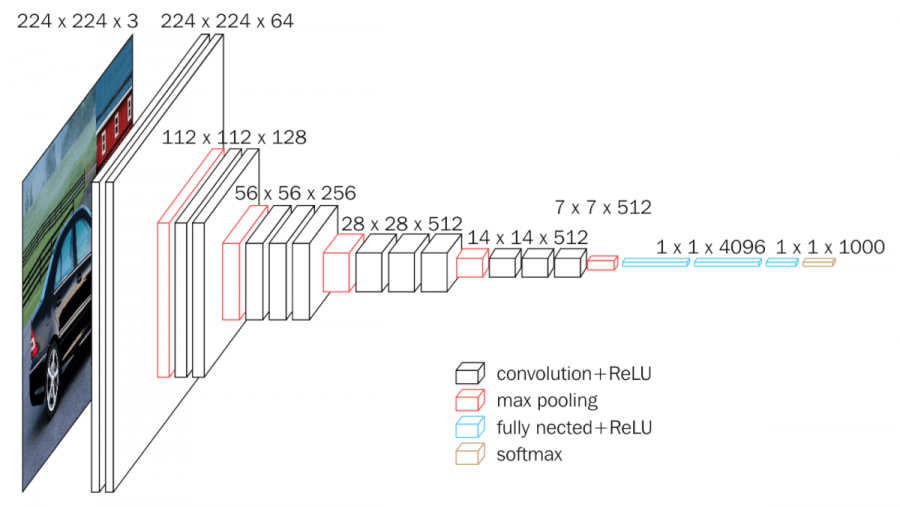
\includegraphics[width=0.8\textwidth]{Figures/vgg16}
  \caption{Structure of the VGG16 network.}%
  \label{fig:vgg16}
\end{figure}
This network was used to classify images with 1000 classes; this is why the
output is $1 \times 1 \times 1000$\footnote{The training data is labelled using
  one-hot encoding. This means the to each image a $1000$ dimensional vector is
  associated where each component corresponds to one class that we want to
  predict and that contains a $1$ in the corresponding entry and is zero
  everywhere else. The network will usually not be 100\% certain about its
  decision and thus the final output of the layer will be a $1000$ dimensional
  vector of which the entries sum to one and which has large values in the
  components that correspond to the predicted classes.}. To gradually reduce the
spatial dimension from $224 \times 224$ to $1 \times 1$, so called max pooling
layers are used.  In this particular case $2 \times 2$ max pooling with a stride
of $2$ was used, which means that the image is partitioned into $2 \times 2$
blocks of which the maximum of the respective four values is taken to replace
this block. The result is a smaller image, more precisely the spatial dimension
is reduced by two in each direction. The effect is visualised in the Figure
below.
\begin{figure}[H]
  \centering 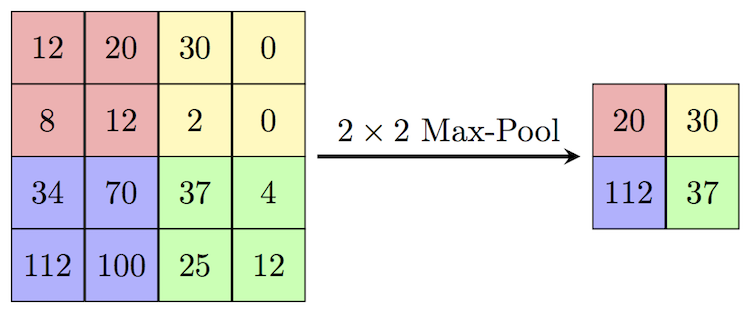
\includegraphics[width=0.6\textwidth]{Figures/maxpool}
  \caption{Effect of a $2 \times 2$ max pool.}%
  \label{fig:maxpool}
\end{figure}
Most layers of the network are convolutional layers with a small receptive field
of $3 \times 3$. For instance, the first two layers after the input layer
consist of 64 distinct convolution filters (typically, in these early layers,
these are edge detectors and the like).

After the stack of convolutional layers, three fully connected layers are
trained. The first two have 4096 channels each, which results in
$4096 \times 4096$ parameters that need to be trained (which is much more than
the number of parameters in the convolutional layers).

The non-linearity used in all of the hidden layers was a rectified linear unit
(ReLU). The last layer consists of a so called softmax function. The goal of
this function is as follows. Prior to applying softmax, some vector components
could be negative, or greater than one; and might not sum to 1; but after
applying softmax, each component will be in the interval $(0,1)$ and the
components will add up to 1, so that they can be interpreted as
probabilities. Furthermore, the larger input components will correspond to
larger probabilities.

\section{Training of a Neural Network: Optimisation}%
\label{sec:train_cnn}
When we have decided on which architecture we want to use (cf.~the last
chapter), we can start to train the network. We begin by initialising the
weights randomly which will obviously not generate any meaningful results.  The
goal is now to (iteratively) find a set of weights that correspond to a
better-performing network, or in other words weights that correspond to a lower
loss. Most modern network use the (stochastic) gradient descent algorithm to
minimise the loss function. To find a minimum of a function starting from a
random point on the graph, we can go in the direction of a negative gradient.
This is the basic idea of gradient descent. At each step in learning we go one
step in the direction of a negative gradient; of course theoretically the
derivative only guarantees that the function will decrease if we take an
infinitely small step which is obviously not possible in practice. The ``size''
of the step is a hyper-parameter called the learning rate which has to be
adjusted beforehand.

In classic gradient descent, we would do this for every image in the training
set which is usually very inefficient. Especially in the beginning, where the
weights have random values, it is not necessary to incorporate every training
image in computing the next (small) step towards a minimum. Therefore we only
optimise over so called mini-batches of the dataset which are usually chosen
randomly from the set of training images. The size of the mini-batch is another
hyper-parameter that has to be chosen before training; usually batches are not
larger than 100 (in some contexts only the extreme case of mini-batches
consisting o a single image is called stochastic gradient descent; sometimes
also mini-batch gradient descent is referred to as stochastic gradient descent).

\section{Convolutional Neural Networks for Semantic Segmentation}
The goal of semantic segmentation is to understand what is in an image on a
pixel level, \ie to assign a class to each pixel in an image. This is visualised
in the following image which is taken from the CityScapes dataset.
\begin{figure}[H]
  \centering 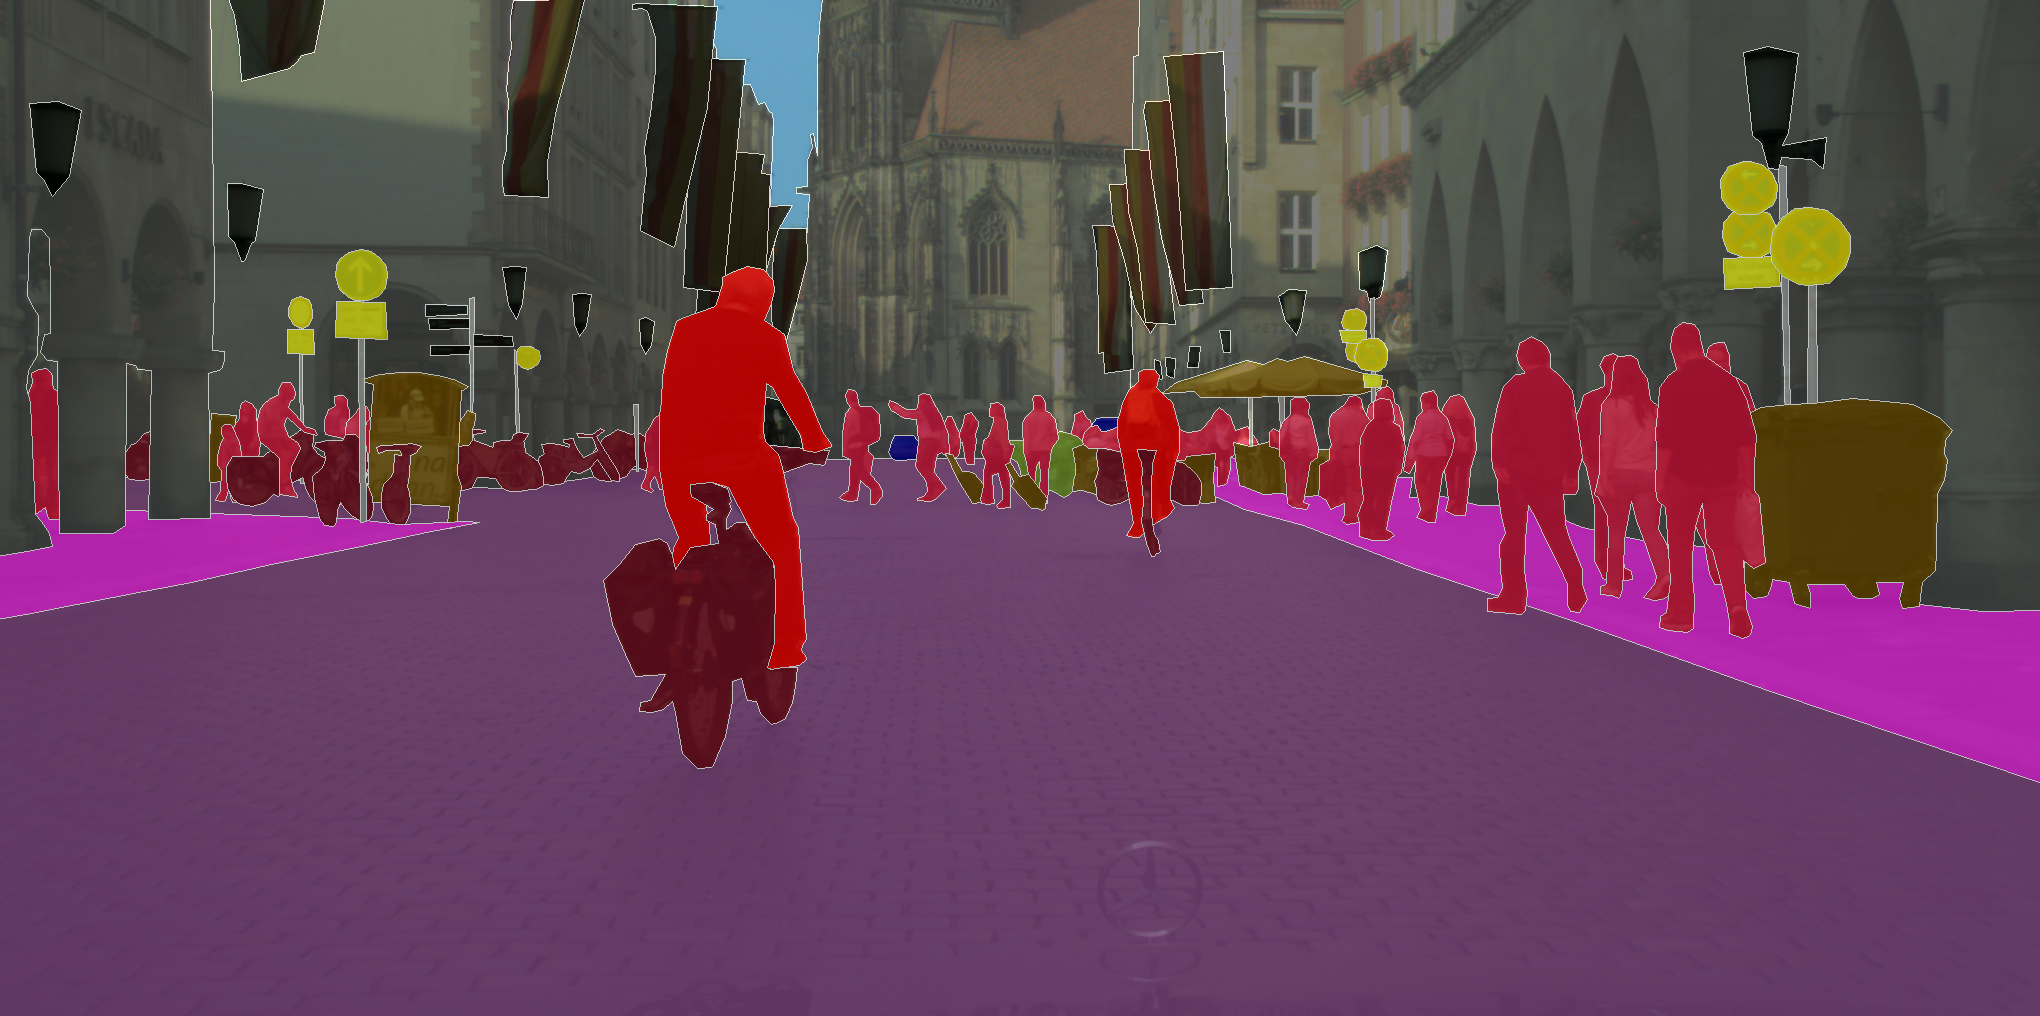
\includegraphics[width=0.7\textwidth]{Figures/cityscapes}
\end{figure}
Another application of semantic segmentation is pose estimation. Here, the
network is asked to find, for instance, all left hands in an image, or all right
feet etc.

One very famous and very successful architecture of a CNN for semantic
segmentation is the UNet given in Figure~\ref{fig:unet}.
\begin{figure}[htpb]
  \centering 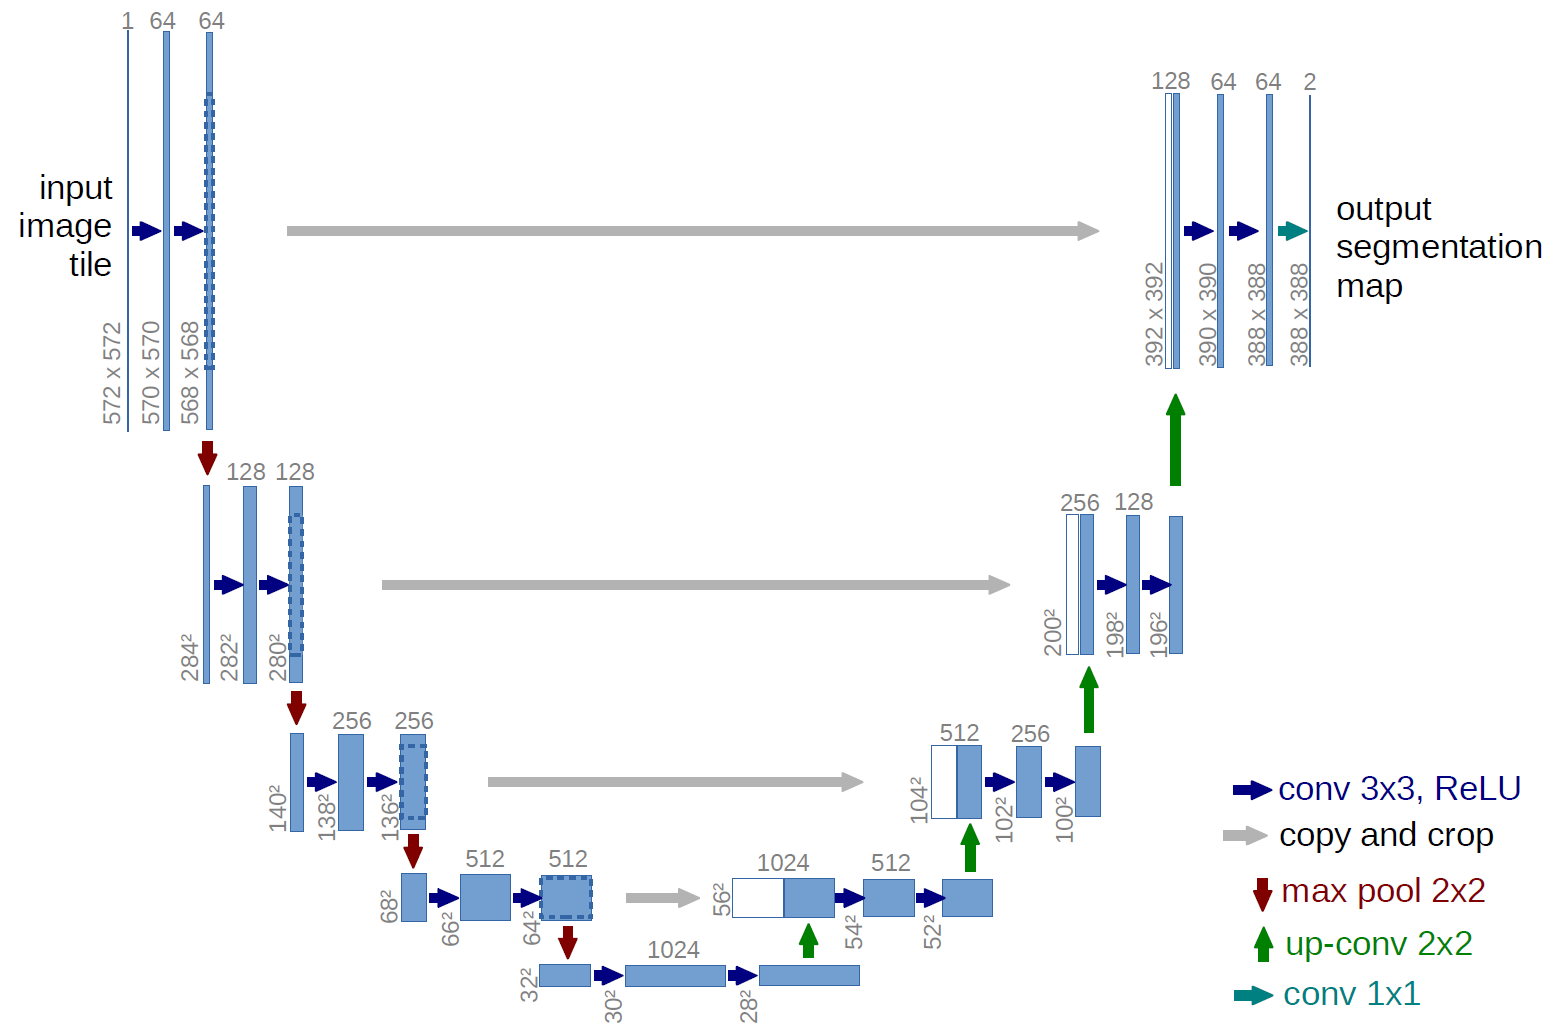
\includegraphics[width=0.7\textwidth]{Figures/unet}%
  \caption{Architecture of the UNet}%
  \label{fig:unet}
\end{figure}
One main difference when compared to the networks we previously discussed is
that some layers or not only connected to the previous layer but also to other
layers. More precisely, the output of some of the early layers is fed into the
corresponding late layer of the same resolution. Further, instead of using max
pool to reduce the dimensions of the image, smoothing and downsampling
convolutional filters are used. They are not prespecified to a certain filter
but are also learned. Similarly, upsampling convolution filters are used to
increase the dimension again. The approach of the UNet can be interpreted as
follows. The layers on the bottom in the Figure are very low-resolution but have
many channels (up to 2014). The path through these layers is therefore referred
to as the semantic pathway. Due to the high number of channels, its aim is to
learn \emph{what} is in each part of the image. However, the low resolution of
$\sim 30 \times 30$ prohibits the network form learning exactly \emph{where}
these things are (for example in the CityScapes dataset, the network might be
very certain that somewhere in the left side of the image there is a tram but it
is unable to exactly pin down its location). This is where the skip connections
(gray, from left to right) come into play. Although they obviously have not yet
understood the difference between, \eg, a tram and a pedestrian, they have
learned where the boundaries of each of these objects are, as they typically act
as edge detectors. This information from this so called geometric pathway is
then combined with the information from the semantic pathway.

In practice, there are several techniques that should be used to improve the
performance of the UNet. First, one should definitely use some form of
normalisation, either group or batch norm (described below). Also, residual
connections should be used in each of the individual blocks of the UNet.
\todo{Residual connections}

\subsection*{Batch and Group Normalisation}


%%% Local Variables:
%%% mode: latex
%%% TeX-master: "../main"
%%% End:
